\section{Numerical Studies} \label{sec:numstd}  
\subsection{Illustrative Example}
We provide here a toy example to illustrate the upper bound approximation method and the lower bound feasibility procedure. 
For this example

$$A=
\left[
\scalebox{0.5}{%
	\begin{tabular}{ c c }
	$-1$ & $0$  \\ 
	$1$ & $0$  \\  
	$0$ & $-1$ \\
	$0$ & $1$  
	\end{tabular}%
} 
\right] \hspace*{0.25in} b=
\left[
\scalebox{0.5}{%
	\begin{tabular}{ c }
	$-0.5$  \\ 
	$3$ \\  
	$-0.5$ \\
	$3$  
	\end{tabular}%
} 
\right] \hspace*{0.25in} Q_1=
\left[
\scalebox{0.5}{%
	\begin{tabular}{ c c }
	$1$ & $0$  \\ 
	$0$ & $0$  
	\end{tabular}%
} 
\right] \hspace*{0.25in} Q_2=
\left[
\scalebox{0.5}{%
	\begin{tabular}{ c c }
	$0$ & $0$  \\ 
	$0$ & $1$  
	\end{tabular}%
} 
\right] \hspace*{0.25in} L=
\left[
\scalebox{0.5}{%
	\begin{tabular}{ c c }
	$-1$ & $0$  \\ 
	$0$ & $1$  
	\end{tabular}%
} 
\right] \hspace*{0.25in} u^*=
\left[
\scalebox{0.5}{%
	\begin{tabular}{ c }
	$2$  \\ 
	$2$   
	\end{tabular}%
} 
\right]
$$
which corresponds to the quadratic system 
$$F(\vx)=\left[\begin{array}{r} x_1^2-x_1 \\ x_2^2+x_2 \end{array}\right]=\left[\begin{array}{r} 2 \\ 2 \end{array}\right] \hspace*{0.15in} \text{s.t.} \hspace*{0.15in} \Omega_{\vx}=\begin{array}{rcl} 0.5\leq & x_1 & \leq 3 \\ 0.5\leq & x_2 & \leq 3 \end{array} $$

Running the outer bound and lower bound feasibility procedures we arrive at a robustness margin of $1.25$ and $1.249998$ respectively, which correspond to the actual robustness margin of 1.25. 
Graphically we can see $F(\Omega_{\vx})$ with $\vu^*$ in \cref{fig:FOmega}.

\begin{figure}[htp!]
	\begin{center}
		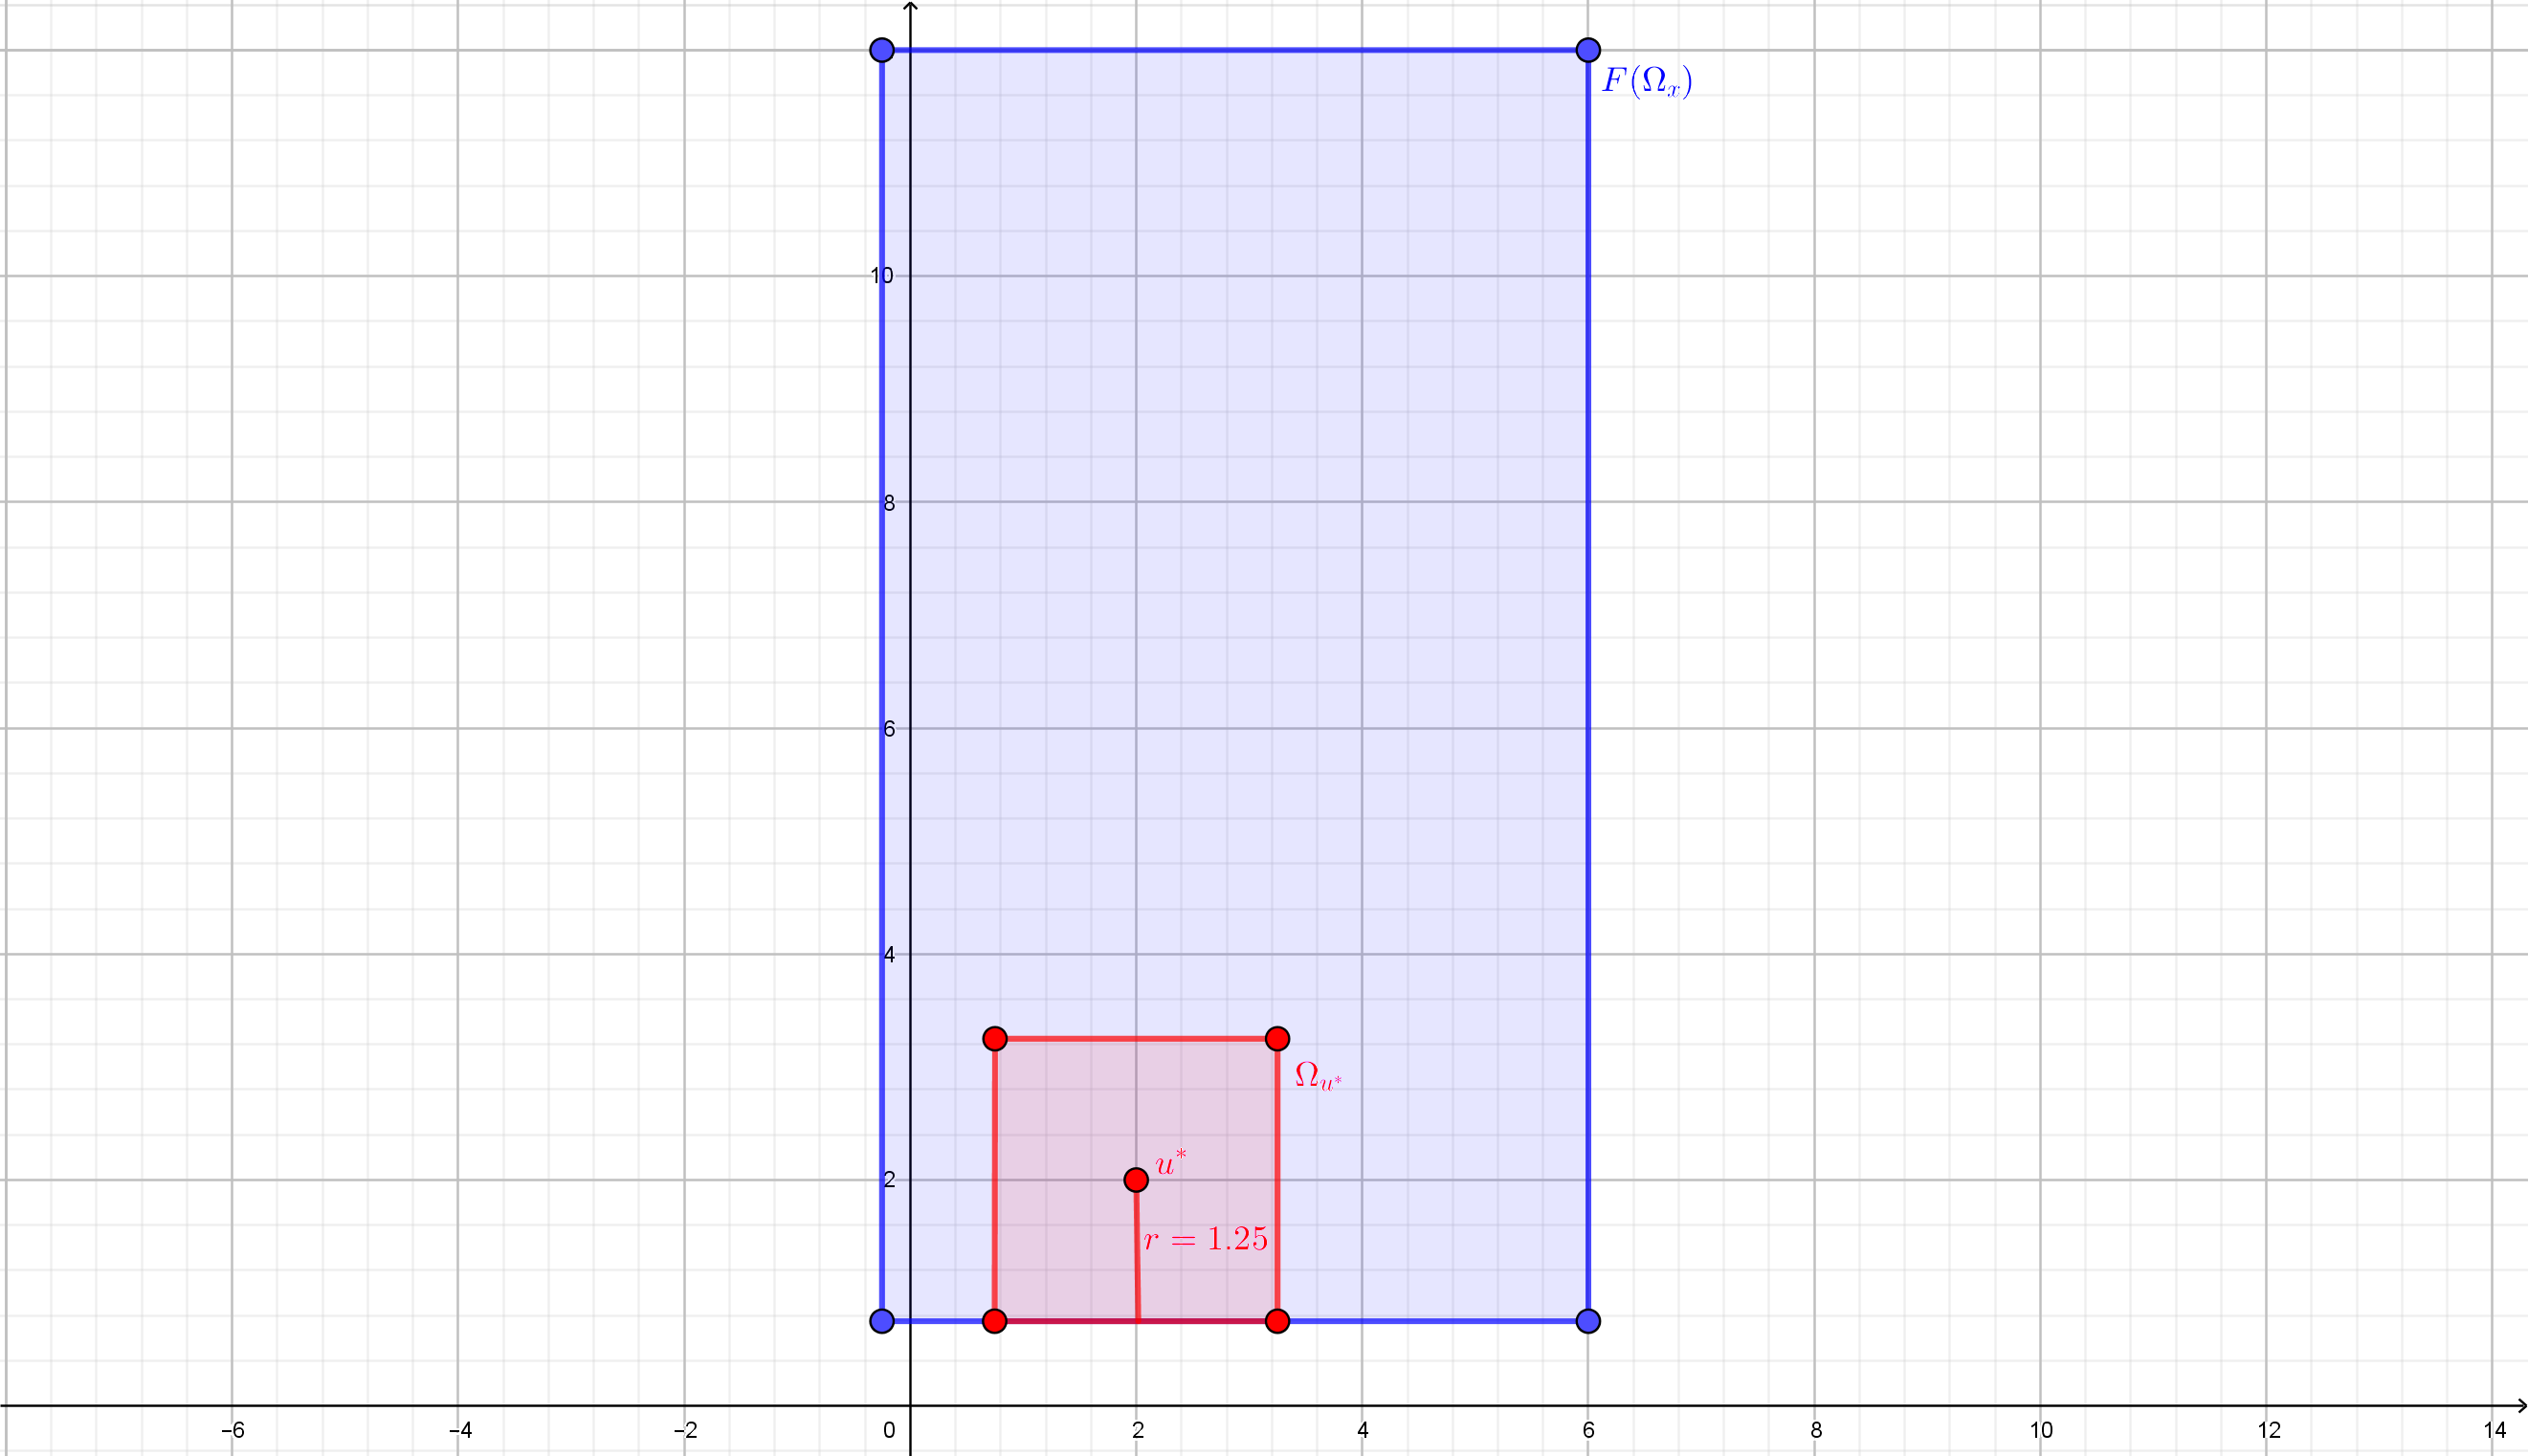
\includegraphics[scale=0.45]{Figures/FOmega2} % {Figures/Rfeas}
	\end{center}
	\caption{Illustration of $F(\Omega_x)$, $u^*$ and $\Omega_{u^*}$.}
	\label{fig:FOmega}
\end{figure}



\subsection{Adaptation to Optimal Power Flow Equations}
Robust feasibility of systems of nonlinear equations has been studied in a series of recent papers \cite{FrKr2015,FrKrWa2016}.
These studies show that the problem is decidable (a terminating algorithm guaranteed to produce an answer exists) as long as the number of variables is not more than twice the number of equations minus $3$.
In our main application domain, we are primarily concerned with the AC power flow equations
%\eqref{eq:ACPF},
where the number of equations is the same as the number of variables, and hence the aforementioned algorithm \cite{FrKr2015,FrKrWa2016} applies to problem \ref{RobustDef}.
However, the algorithm requires computing a simplicial decomposition of the domain set (a triangulation).
The algorithm scales as $\tilde{O}(s^4)$ where $s$ is the number of simplices in the complex.
Further, the number of simplices in a simplicial decomposition grows exponentially with the dimension $n$, severely limiting the scalability of these algorithms to realistically-sized power grids ($n=1000$ or higher).

Specific to power systems, there has been significant empirical work on solving the PF equations with probabilistic uncertainty \cite{morales2007point,wang1992interval}.
However, these algorithms are based on sampling heuristics and do not offer mathematical guarantees of robust feasibility.
There has been recent work on specifying conditions on the power injections over which the power flow equations are guaranteed to have a solution \cite{bolognani2016existence,EPFLA,EPFLB}.
However, they do not directly address the robust feasibility problem, and using these regions to assess robust feasibility can produce very conservative results.
Further, they do not address uncertainty in the quadratic and linear objective terms.

We now present computational studies which support the efficiency of the procedures we have presented, which address the aforementioned short comings of previous work. 
For all the numerical results presented we apply procedures \eqref{eq:OPTfeasOutRelaxb}, \eqref{eq:OPTfeasrelaxLP1}, \eqref{eq:OPTfeasrelaxLP2}, and \eqref{eq:OPTfeasrelaxLP3} to find upper and lower bounds for the robustness margins with respect to the optimal power flow equations derived using datasets obtained from the MatPower package found in the MATLAB software, see \cite{matpower}. 
We will specifically show results for tests conducted on cases 5, 9, 14, 30 and 57. 
In every case the power flow equations were converted into the format defined by \eqref{eq:Quad}, \eqref{eq:xLimits}, and \eqref{eq:uLimits}. 
To simulate real life scenarios we allowed the first 5 dimensions of $\vu$ to represent renewable energy, and the others representing no variation. We then slowly increased the variation of the first 5 dimensions of $\vu$, while utilizing procedures \eqref{eq:OPTfeasOutRelaxb} for the outer bound, and \eqref{eq:OPTfeasrelaxLP1}, \eqref{eq:OPTfeasrelaxLP2} and \eqref{eq:OPTfeasrelaxLP3} for the inner bound verification to verify robust feasibility. 
The following subsection will detail specifically how this transformation was conducted.

\subsubsection{OPF to Quadratic System}
As described in \cite{DjTuritsyn}, the AC power flow equations can be written as 
\begin{equation}\label{eq:Real1}
	\begin{array}{rl}
	Re\left(\sum\limits_{k=1}^n V_i\left(\overline{Y_{ik}V_k} + \overline{Y_{i0}V_0}\right)\right) &= p_i \ \forall i\in PQ \\
	
	Im\left(\sum\limits_{k=1}^n V_i\left(\overline{Y_{ik}V_k} + \overline{Y_{i0}V_0}\right)\right) &= q_i \ \forall i\in PQ \\
	
	Re\left(\sum\limits_{k=1}^n V_i\left(\overline{Y_{ik}V_k} + \overline{Y_{i0}V_0}\right)\right) &= p_i \ \forall i\in PV \\ 
	
	|V_i|^2 &= v_i, \  \ \forall i \in PV 
	\end{array}
\end{equation}

%\begin{align*}\label{eq:Real1}
%& Re\left(\sum\limits_{k=1}^n V_i\left(\overline{Y_{ik}V_k} + \overline{Y_{i0}V_0}\right)\right) = p_i \ \forall i\in PQ \\ \nonumber
%& Im\left(\sum\limits_{k=1}^n V_i\left(\overline{Y_{ik}V_k} + \overline{Y_{i0}V_0}\right)\right) = q_i \ \forall i\in PQ \\ \nonumber
%& Re\left(\sum\limits_{k=1}^n V_i\left(\overline{Y_{ik}V_k} + \overline{Y_{i0}V_0}\right)\right) = p_i \ \forall i\in PV \\ \nonumber
%& |V_i|^2 = v_i, \  \ \forall i \in PV 
%\end{align*}
%%
where $V_i$ denotes the complex voltage phasor, $p_i$ the active and $q_i$ the reactive power injection, and $Y$ the admittance matrix at node $i$. $PV$ denotes the set of $PV$ nodes, $PQ$ denotes the set of $PQ$ buses and $v_i$ denotes the squared voltage magnitude setpoints at the $PV$ buses. We can then rewrite \cref{eq:Real1} into the system outlined by \cref{eq:Quad}, \cref{eq:xLimits}, and \cref{eq:uLimits} with 
\[
\begin{array}{rl}
\vx= & \begin{bmatrix} Re(V_1) & \dots & Re(V_n) & Im(V_1) & \dots  &  Im(V_n) \end{bmatrix}^T ~~\mbox{and} \\
\vu=& \begin{bmatrix} p_1 &  \dots &  p_n &  q_1 &  \dots &  q_n &  v_1 &  \dots &  v_n \end{bmatrix}^T.
\end{array}
\]



\subsubsection{Computational Results}


The procedures were conducted with $A\vx \leq \vb = B \vone$ for $B\in\{0.001, 0.005,0.01\}$.
$A$ in this cases is a matrix s.t. $A\vx \leq \vb$ controls the flow between nodes in the power grid (i.e. each row of $A\vx \leq \vb$ has the form $x_i-x_j\leq b_k$. 
All computations were performed on a laptop running the 64bit Windows 10 operating system containing an Intel i-7 processor, 16 GB of Ram and 4 cores. 
Graphically we can look at this data on a case by case basis to highlight the effect of allowing more fluctuation between the nodes (i.e. as $B$ increases).(Figure \ref{fig:Graphs1}) 

\begin{figure}[htp!]
\begin{center}
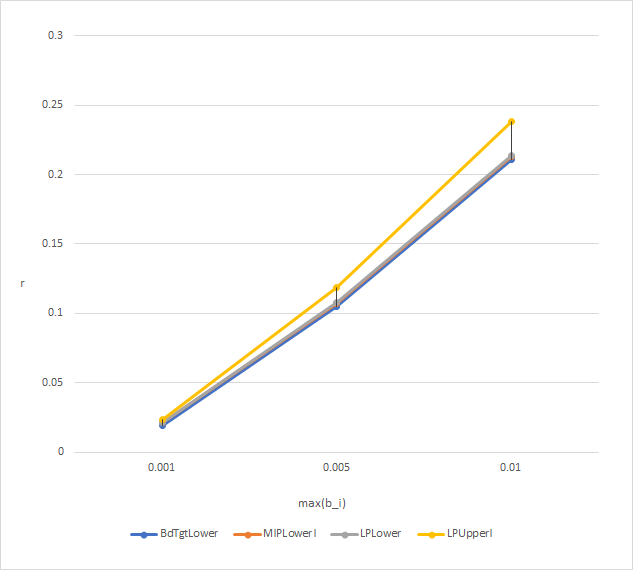
\includegraphics[scale=0.45]{Figures/Case5}
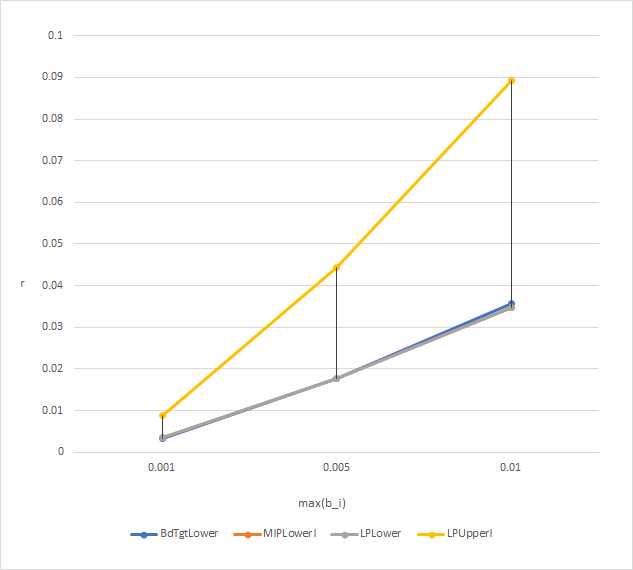
\includegraphics[scale=0.45]{Figures/Case9} \\
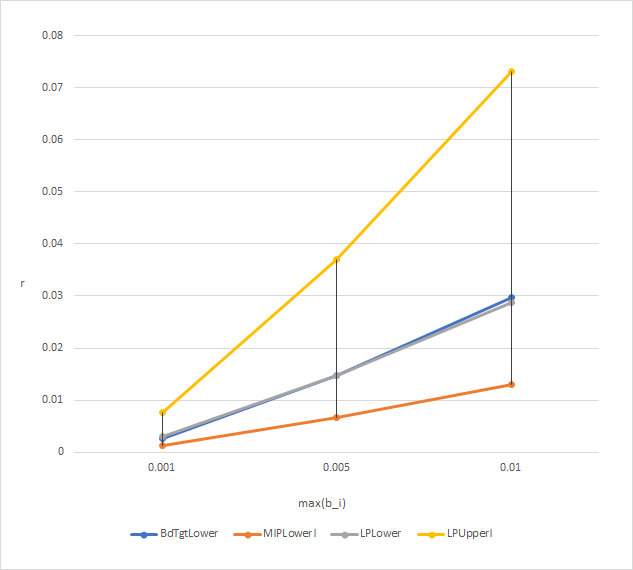
\includegraphics[scale=0.45]{Figures/Case14}
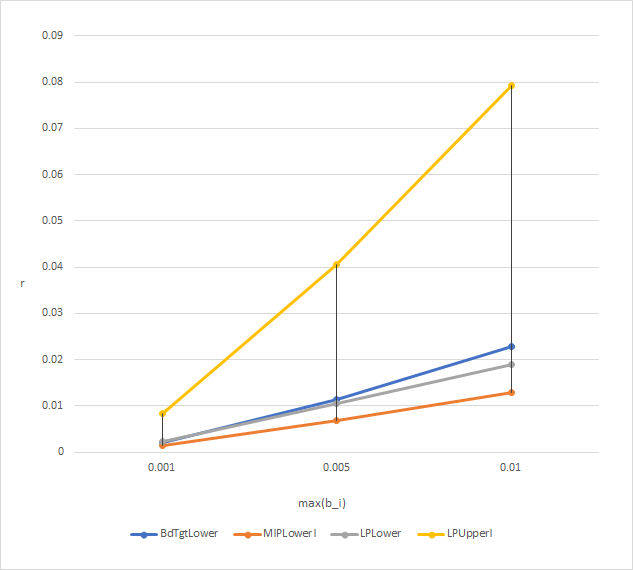
\includegraphics[scale=0.45]{Figures/Case30}
\caption{Case 5 (Top Left), Case 9 (Top Right), Case 14 (Bottom Left), Case 30 (Bottom Right)} 
\label{fig:Graphs1} 
\end{center}
\end{figure}

Case 57 is not included in the graphs as the only inner bound procedure to run in any reasonable time was the Feasibility procedure that produced a max robust margin of $\approx$0.003 with a computational time of $\approx$489224 and a gap to the outer bound procedure, which had a running time $\approx$45144, of $\approx 0.030$ when $B=0.001$.
As evident from the graphs we have that the bound tightening procedure produces a better approximation of the inner bound on the robustness margin as the complexity of the data set increases. 
Certainly one would expect the bound tightening procedure to out perform the other inner bound procedures for all cases, but the choice of procedure parameters has a big effect on the efficiency of the procedure. 
For instance, setting a low tolerance for a minimal sufficient change in the dimensions of $\vb$ will cause in most cases an extremely long running time. 
Thus in the extremely low and marginally high complexity cases it should be expected that the other procedures will out perform the bound tightening procedure as these manually set parameters will have more of an impact on performance. 
Of special interest is the difference in performance of the MIP and Feasibility inner bound procedures as the complexity of the data increases. 






